{\Large John \sc Gliksberg}
\hrulefill\\[-.47cm]
\begin{minipage}{0.8\textwidth}
\begin{flushleft}
\vspace{.5cm}
21 ans, né le 25 juin 1994\\
14 rue Anatole France, 92310 Sèvres\\[.2cm]
06 40 60 76 95\\
\href{mailto:jg.trosh@gmail.com}
{jg.trosh@gmail.com}\\[.2cm]
Langues maternelles français \& anglais\\
Permis B, véhicule personnel
\end{flushleft}
\end{minipage}%
\begin{minipage}{0.2\textwidth}
\begin{figure}[H]
\begin{flushright}
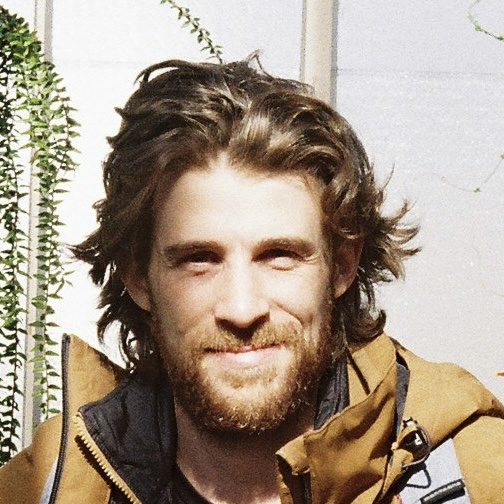
\includegraphics[height=3cm]{johnpic}
\end{flushright}
\end{figure}
\end{minipage}\\

\begin{center}
    \framebox{
        \parbox{335\unitlength}{
            \centering\large\sc
            Recherche stage de 6 mois de fin d'études \\
            M2 Informatique Haute Performance \& Simulation
        }
    }
\end{center}
\vspace{.3cm}

{\large\bf Profil}
\hrulefill\\[.3cm]
{\setlength{\extrarowheight}{.2cm}
Je suis très motivé, adaptable et ai développé une approche responsable
dans toutes les tâches que j'entreprends.
Mes managers et superviseurs apprécient la fiabilité de mes analyses
et ma capacité de compréhension et de résolution de problèmes techniques.
Je suis avide de découvertes, autant prêt à travailler en équipe que
de mon initiative, en français autant qu'en anglais.
}
\vspace{.3cm}

{\large\bf Études}
\hrulefill\\[.3cm]
{\setlength{\extrarowheight}{.2cm}
\begin{tabularx}{\textwidth}{lX}
2015 \---- 2016 &
\href{http://mihps.prism.uvsq.fr}
{\bf Master 2 Informatique Haute Performance \& Simulation}
\newline
Université de Versailles Saint-Quentin-en-Yvelines (UVSQ) \\
2015 &
\href{http://mihps.prism.uvsq.fr}
{\bf Master 1 Informatique Haute Performance \& Simulation}
(mention bien, major)
\newline
Université de Versailles Saint-Quentin-en-Yvelines (UVSQ) \\
2014 &
\href{http://www.uvsq.fr/double-licence-mathematiques-et-physique-343617.kjsp}
{\bf Double Licence Mathématiques \& Physiques}
\newline
Université de Versailles Saint-Quentin-en-Yvelines (UVSQ) \\
2011 &
\href{http://www.education.gouv.fr/cid20999/l-option-internationale-du-baccalaureat-o.i.b.html}
{\bf Baccalauréat Scientifique OIB} (option internationale)
\newline
Lycée de Sèvres (SIS) \\
2010 &
\href{http://www.cambridgeenglish.org/exams/proficiency/}
{\bf Certificate of Proficiency in English} (CPE)
\---- {\bf Anglais niveau C2}
\newline
University of Cambridge
\end{tabularx}}
\vspace{.3cm}

{\large\bf Portfolio}
\hrulefill\\[.2cm]
Langages : C, C++, Python 2/3, Lua, Go, Scilab, Matlab, Fortran, Cuda \\
Librairies : Blas, Lapack, Vtk, MPI, OpenMP \\
Outils : Linux, bash/zsh, vim/emacs, Paraview, Makefile, \LaTeX, git/svn \\
Misc : html/css, js, php, sql
\vspace{.3cm}

{\large\bf Activités professionnelles}
\hrulefill\\[.2cm]
{\setlength{\extrarowheight}{.2cm}
\begin{tabularx}{\textwidth}{lX}
2015 &
\href{http://www.scilab-enterprises.com}
{\bf Scilab-Enterprises}, Versailles
\newline
Stage de 4 mois à temps complet \---- développeur logiciel open-source
\newline
Industrialisation de modules Scilab, développements sur Scilab 6
\\
2014 &
Laboratoire de physique
\href{http://www.gemac.uvsq.fr/}
{\bf GEMaC\--CNRS\--UVSQ}, Versailles
\newline
Stage de 4 mois à temps partiel
\newline
\og Étude visuelle de transitions de phase dans des monocristaux\fg
\\
2013 \---- 2015 &
Tuteur et formateur en anglais,
\href{http://www.cerel.uvsq.fr/presentation-291090.kjsp}
{\bf CEREL \makeatletter @ \makeatother UVSQ} \newline
Tutorats en groupes \----
Cours individuels pour étudiants malentendants
\end{tabularx}}
\vspace{.3cm}

{\large\bf Autres activités}
\hrulefill\\[.3cm]
{\setlength{\extrarowheight}{.15cm}
\begin{tabularx}{\textwidth}{lX}
2014 \---- 2015 &
Coordinateur et co-fondateur de l'association
\href{https://www.facebook.com/pages/Seventy-Eighters/508772502567015}
{Seventy-Eighters}
\makeatletter @ \makeatother UVSQ \\
2013 \---- 2015 &
Élu étudiant au Conseil UFR
\makeatletter @ \makeatother UVSQ
\end{tabularx}}
\newline
{\setlength{\extrarowheight}{.15cm}
\begin{tabularx}{\textwidth}{X}
Dessin (portraits, bande-dessinée) \hfill
Lecture, cinéma (SF) \hfill
Tennis de table \\
Musique (électronique, bossa nova, jazz) \hfill
Projet Euler \hfill
Animation procédurale
\end{tabularx}}
